\subsection{Translating Embeddings (TransE)}
Commonly used benchmark, and one of the first KGE models.
This approach attempts to model relationships as translations between two points (nodes) in a vector space

Given a statement $s = (h,r,t)$, ideally $h$ and $t$ should be close to each other in the vector space,
with the difference being the translation of the relation $r$~\cite{TransE}.


\begin{figure}[h] % [h] attempts to place figure here, other options like [t]op, [b]ottom
    \centering % Centers the figure horizontally
    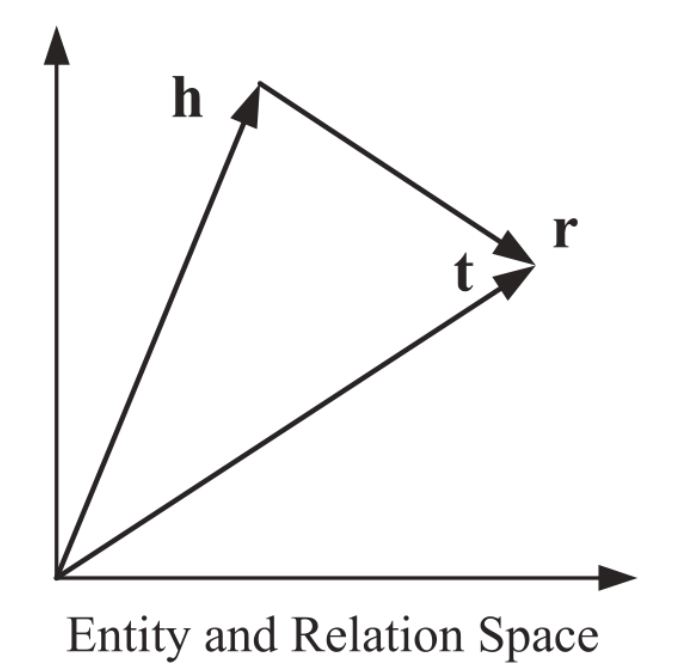
\includegraphics[width=0.35\linewidth]{figures/transe} % Include the image with desired width
    \caption{Visualization of TransE~\cite{TransEFig}}
    \label{fig:transe-example}
\end{figure}.

\FloatBarrier

\subsection{Relational Rotation Embeddings (RotatE)}
"The RotatE model maps
the entities and relations to the vector space and defines each relation as a rotation from
the source entity to the target entity."~\cite{RotatE}

The benefit of RotatE over TransE lies in expressiveness.
It is able to model more relationship patterns, such as symmetry, antisymmetry, inversion
and composition.

\begin{figure}[h] % [h] attempts to place figure here, other options like [t]op, [b]ottom
    \centering % Centers the figure horizontally
    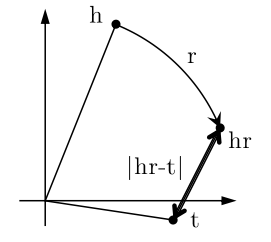
\includegraphics[width=0.35\linewidth]{figures/rotate} % Include the image with desired width
    \caption{Visualization of RotatE~\cite{RotatE}}
    \label{fig:rotate}
\end{figure}.

\FloatBarrier


\subsection{Holographic Embeddings (HolE)}

Holographic Embedding~\cite{HolE} is a model for learning representations of entities and relationships in a knowledge graph.
It uses the principles of holography and circular correlation to combine entity embeddings in a way that captures rich
interactions between entities and relations.

The main benefit of HolE over other approaches is the increased modeling power.

\subsection{The Bilinear Diagonal DistMult Model (DistMult)}

DistMult is a tensor factorization based model introduced in~\cite{DistMult} that uses,
trilinear dot product as its scoring function.

However, a big limitation of DistMult is that it cannot model asymmetric relationships.

\subsection{Complex Embeddings (ComplEx)}

ComplEx~\cite{ComplEx} is similar to DistMult in using the dot product of two vectors to calculate the score.
However, it uses the Hermitian dot product, which is able to handle asymmetrical relationships.

Moreover, instead of using real-valued vectors, DistMult uses a complex vector space for both entities and relations.
Allowing to capture richer information about the graph at the cost of increased computational cost.

\subsection{Benchmark Comparison of KGE Methods}
Table~\ref{tab:kge-perf-comp} shows the performance of the above-detailed KGE methods on the FB15k benchmark dataset.


\begin{table}[!ht]
    \centering

    \begin{tabular}{|l|l|l|l|}
        \hline
         & MRR            & Hits@1                       & Hits@10               \\ \hline
TransE   & 0.463          & 0.29                         & 0.75                  \\ \hline
RotatE   & 0.797          & \textbf{0.746}               & 0.884                 \\ \hline
HolE     & 0.524          & 0.4                          & 0.73                  \\ \hline
DistMult & \textbf{0.841} &                              & \textbf{0.914}        \\ \hline
ComplEx  & 0.84           & 0.692 &  0.75                                        \\ \hline
\end{tabular}
\caption{Performance of Discussed KGE Methods on the FB15k Benchmark Dataset. Datasources~\cite{paperswithcode2024fb15k, HolE}}
\label{tab:kge-perf-comp}
\end{table}
